\documentclass{beamer}
\usepackage{scuwqt}
\usepackage{booktabs}
\setlength\parindent{2em}
\renewcommand{\arraystretch}{1.5}
\setCJKfamilyfont{font01}{AR PL KaitiM GB}
\newcommand{\fonta}{\CJKfamily{font01}}
%=========================================================
\title{Title here}
\author{Candidate:  \ Advisor :}
\institute{College of xxxx at Sichuan University}
\date{\today}
\setlength{\parindent}{2em}
\setbeamertemplate{background}{%
\tikz[overlay,remember picture]{
    \ifnum\thepage=1
        \node[at=(current page.north),anchor=north,yshift=0.3cm] {
            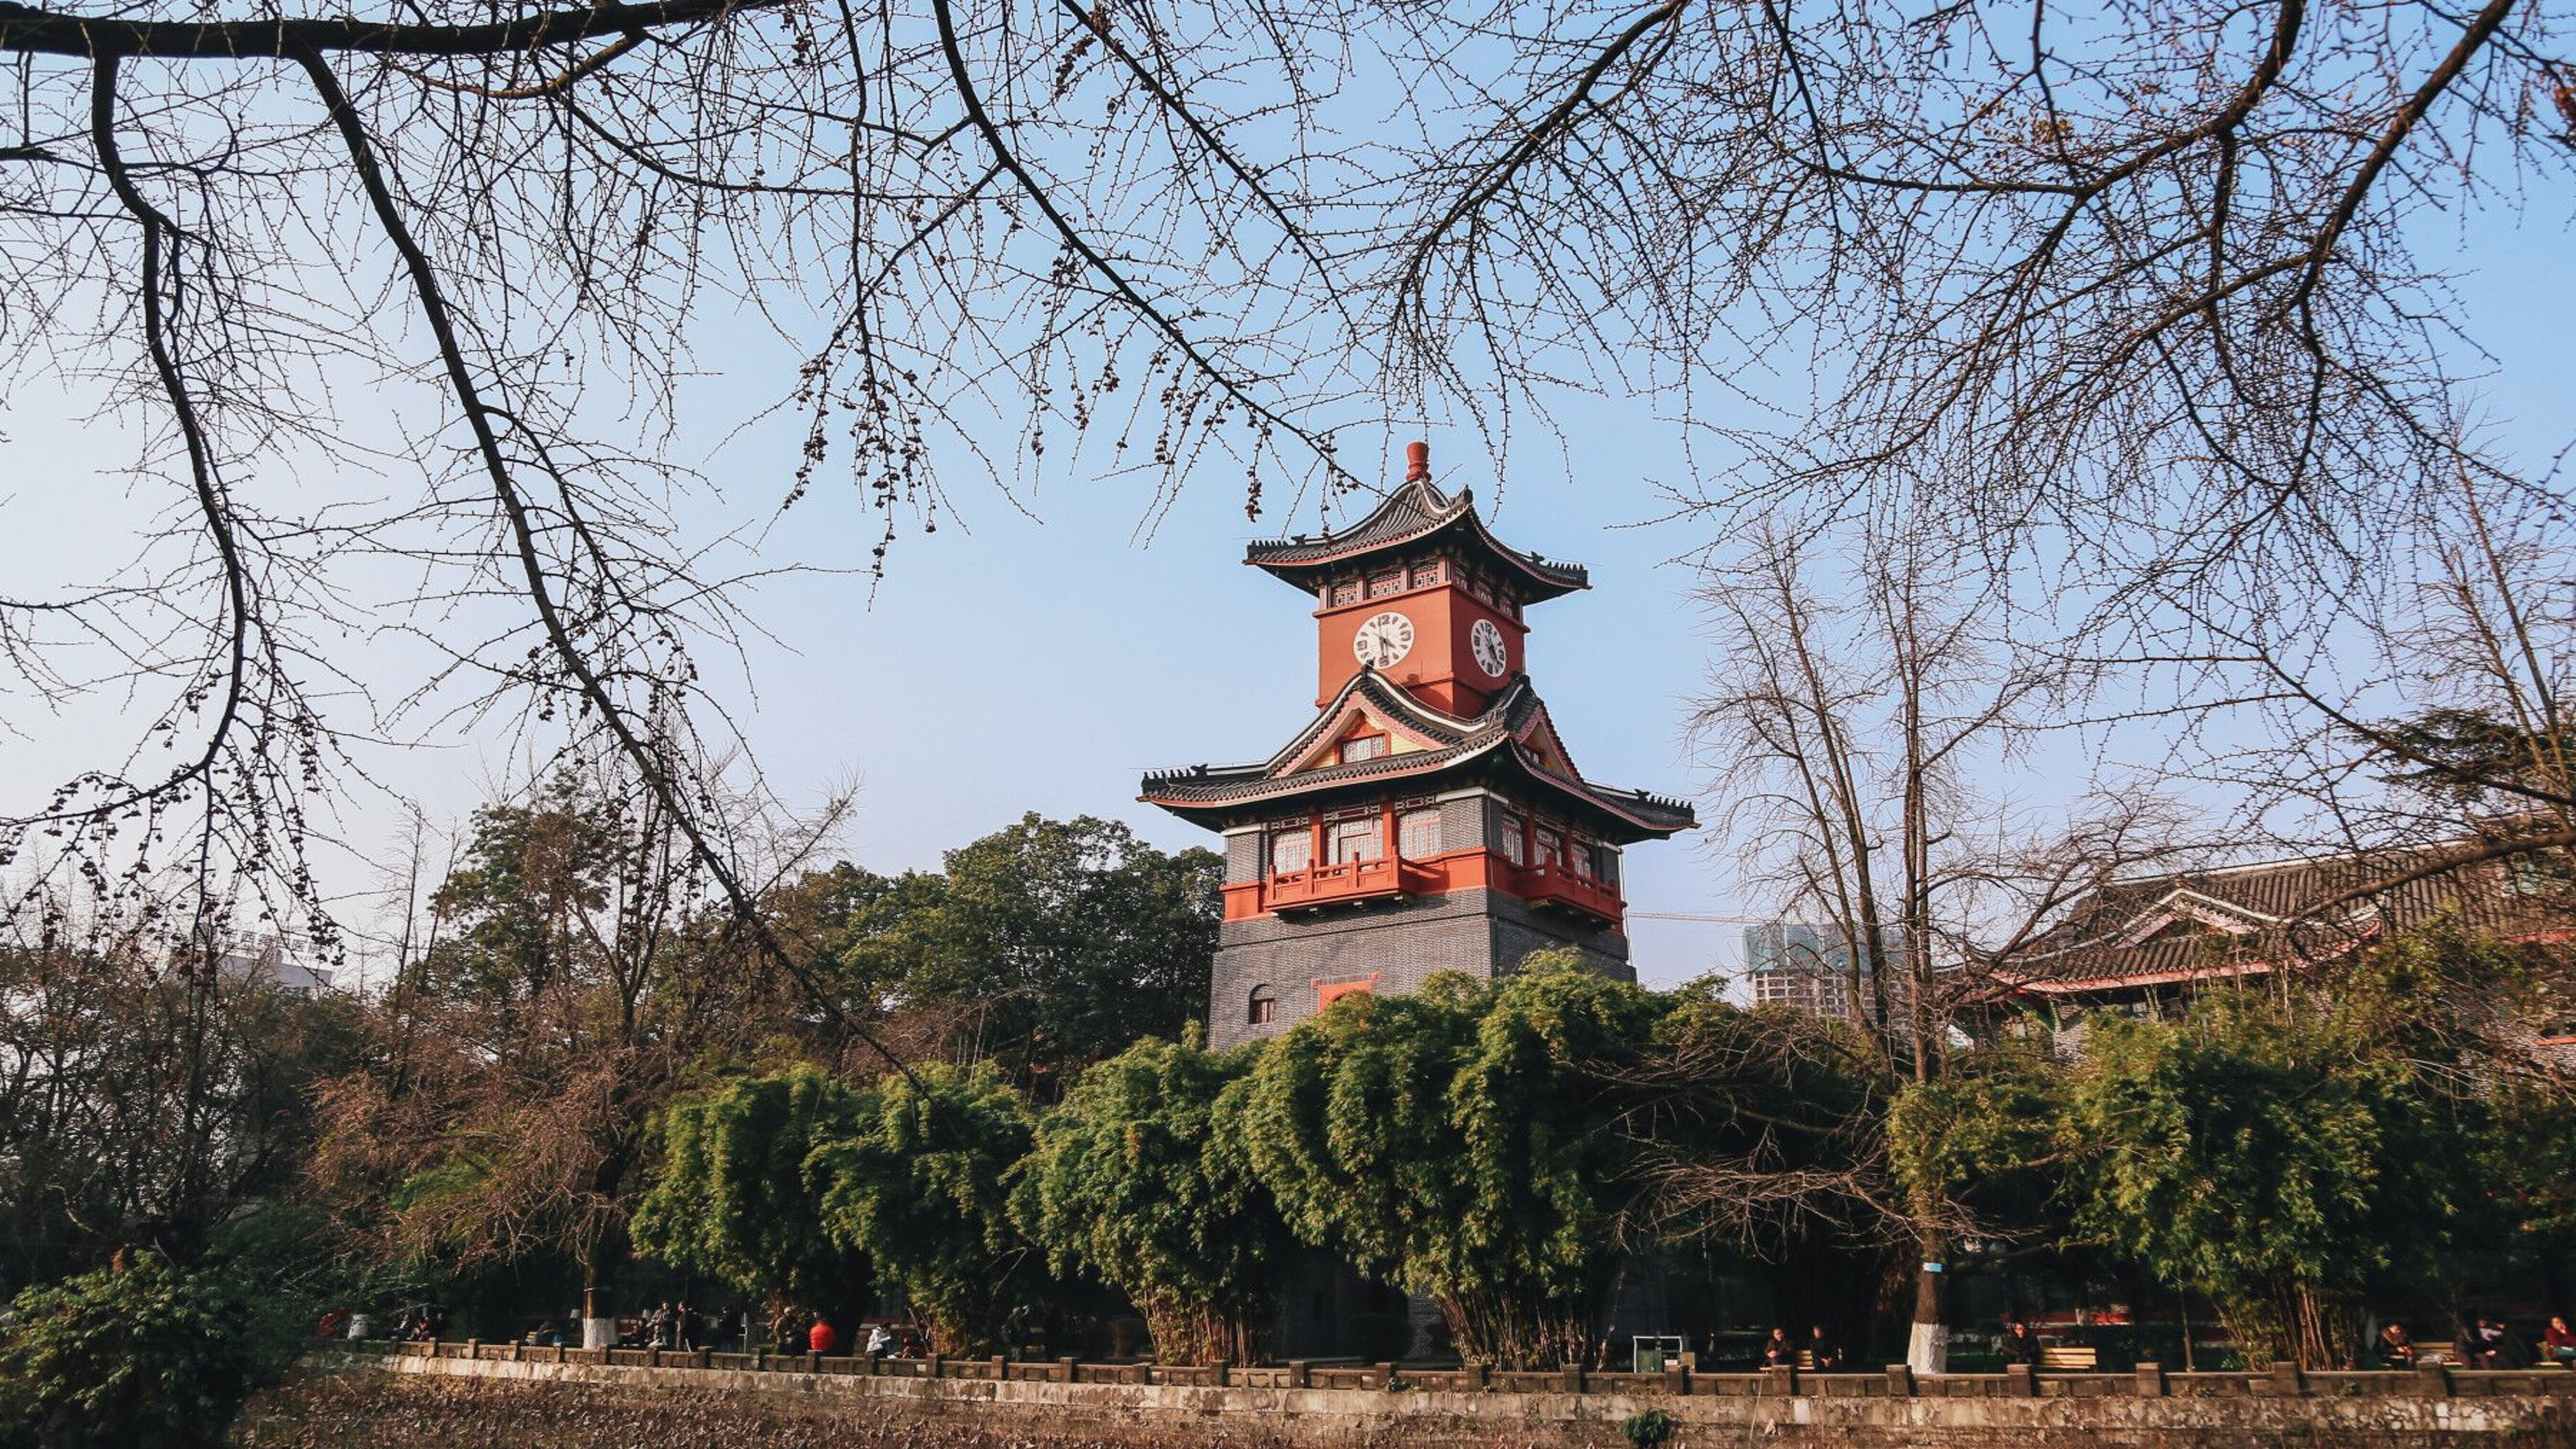
\includegraphics[width=\paperwidth,height=0.7\paperheight]{background.jpg}
        };
    \else
        \node[at=(current page.south west), anchor=south west, xshift=0.1cm, yshift=0.3cm] {
            
\includegraphics[width=2cm]{logo.png}
        };
    \fi
}

    }%设置基本的背景
\begin{document}
{

\begin{frame}
  \titlepage
\end{frame}
%=========================================================
{
    \usebackgroundtemplate{
        \tikz\node[at=(current page.west), yshift=-3cm]  {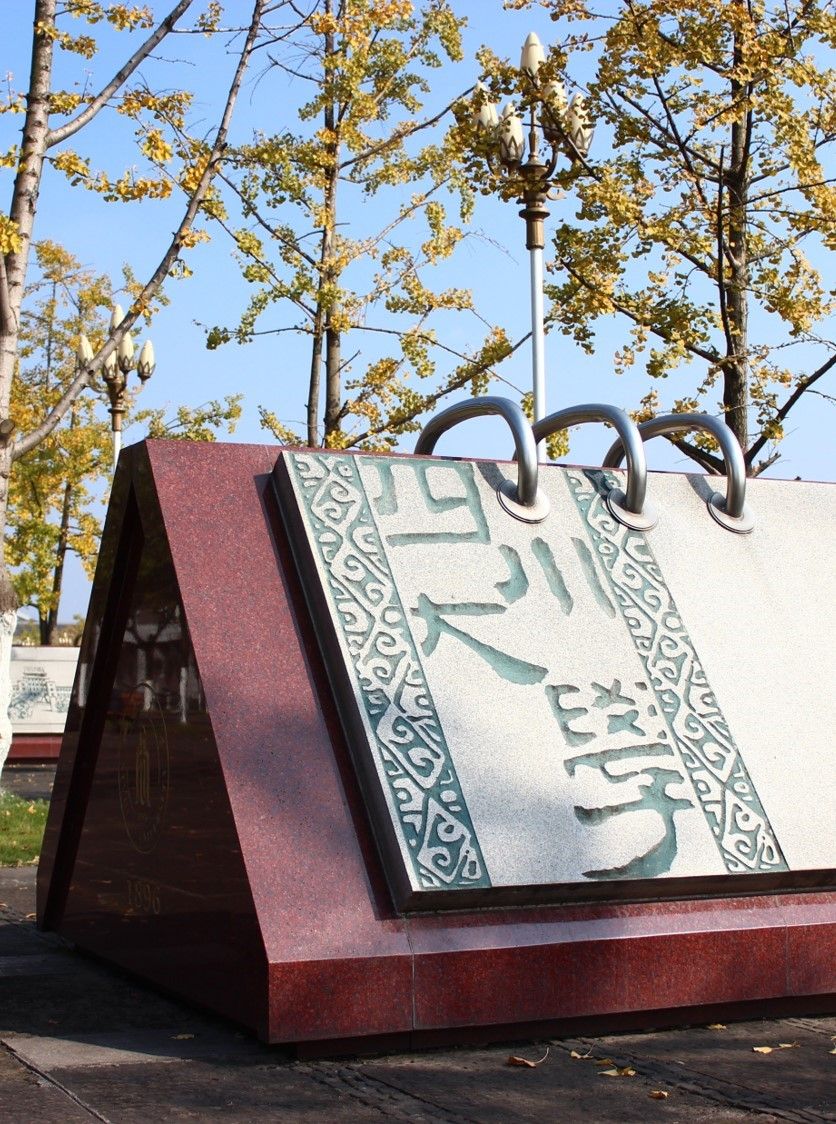
\includegraphics[width=0.5\paperwidth,height=\paperheight]{contents.jpg}};
    }

\begin{frame}

  \hfill % 使用 \hfill 来推动内容到右侧
  \begin{minipage}[t]{.4\textwidth} % 创建一个宽度为文本宽度一半的 minipage,你可以根据需要调整这个宽度
    \tableofcontents % 将目录放在这个 minipage 中
  \end{minipage}
\end{frame}}
%=========================================================

\section{Introduction}

\begin{frame}
  \frametitle{Introduction}
\begin{columns}[T]
    \begin{column}{0.6\textwidth}
\setlength{\parindent}{2em}
Overleaf现有的四川大学演示模板配图、色调欠缺。

\begin{itemize}
\item 编译环境:Texlive(XeLatex)\url{https://www.tug.org/texlive/}
\item Github:\url{https://github.com/WQT1123/SCU-Presentation-Beamer}
\item 私信方式:2637288021@qq.com
\end{itemize}
\large Tips:
建议搭配GPT4(极速水PPT)(doge):\url{https://chat.openai.com/g/g-tDi9X7Pjd-latex-ppt}
    \end{column}
    \begin{column}{0.4\textwidth}
      \begin{figure}[t]
        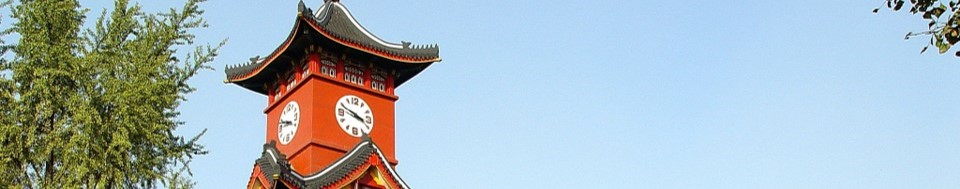
\includegraphics[width=0.8\linewidth,height=0.3\textheight]{background1.jpg}
        \caption{备选背景}
      \end{figure}
\vspace{-0.5cm}
      \begin{figure}
        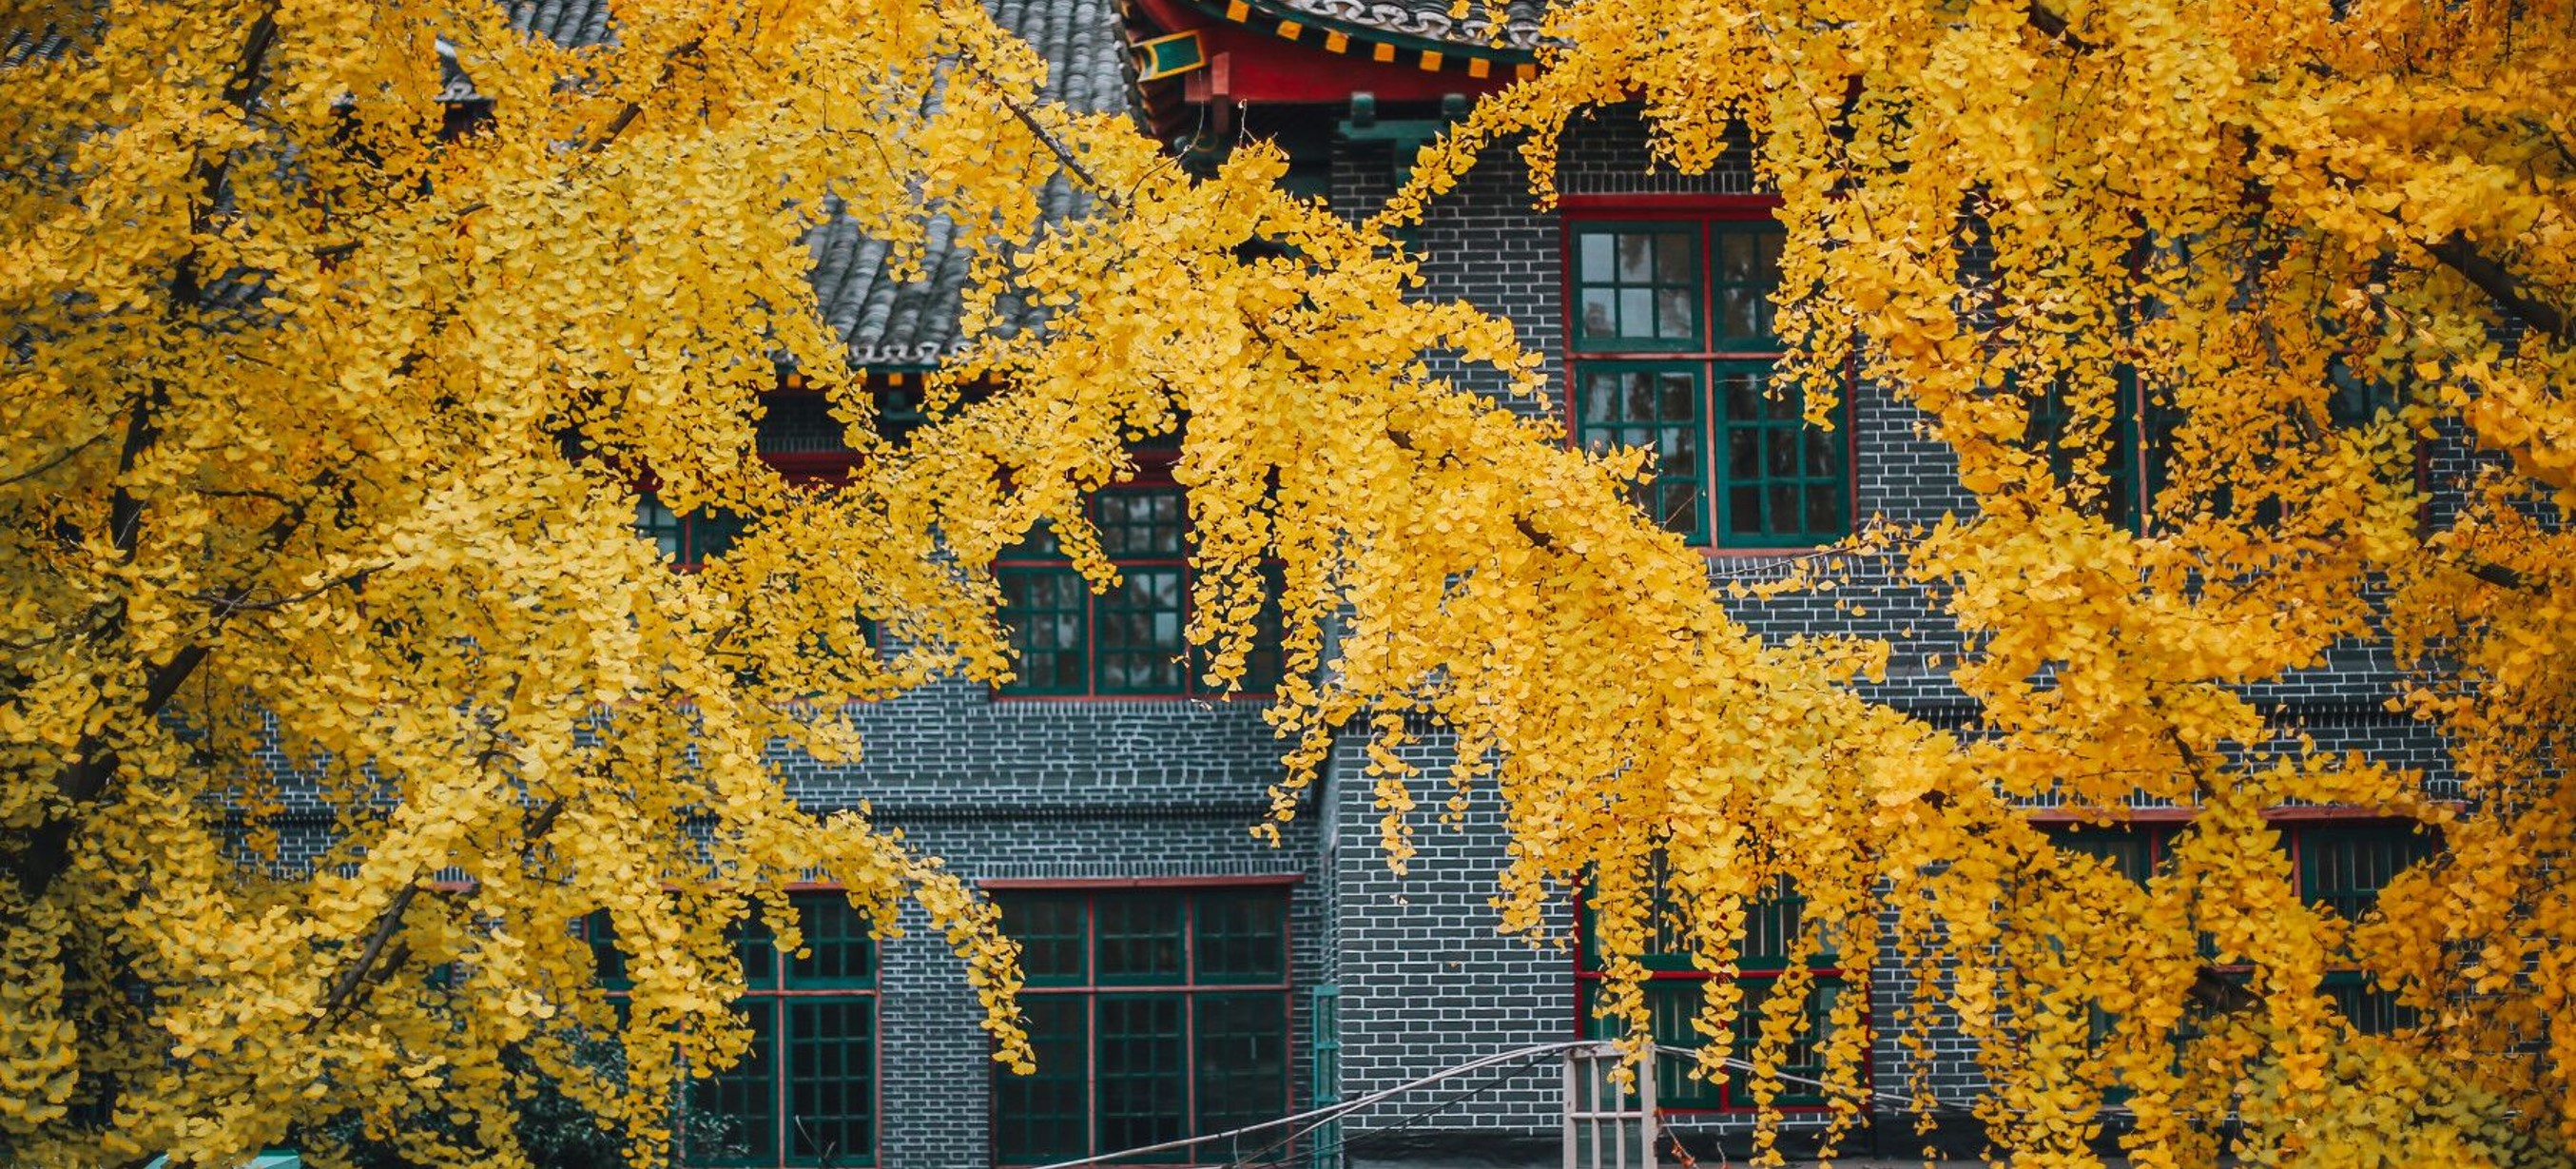
\includegraphics[width=0.8\linewidth,height=0.3\textheight]{end1.jpg}
        \caption{备选结束页插图}
      \end{figure}
    \end{column}

  \end{columns}


\end{frame}
%=========================================================
\section{Research Significance}
\begin{frame}
  \frametitle{Research Significance}

    
\end{frame}
%=========================================================
\section{Technical Route}
\subsection{Technical Route1}
\begin{frame}
  \frametitle{Technical Route1}

\begin{table}[h]
        \centering
        \begin{tabular}{|l|l|}
          \hline
          \textbf{优点} & \textbf{描述} \\
          \hline
          准确性 & 通过精确测量电磁特性进行可靠分类 \\
          \hline
          快速性 & 测量过程快速,适用于大批量样品 \\
          \hline
          无需接触 & 非破坏性测量,不损伤样品 \\
          \hline
          适用性广 & 适用于多种不同类型的材料 \\
          \hline
          经济高效 & 相较于其他方法成本较低 \\
          \hline
        \end{tabular}
        \caption{电磁方法的优点}
      \end{table}
\end{frame}
\subsection{Technical Route2}
\begin{frame}
 \frametitle{Technical Route2}

\begin{table}[h]
        \centering
        \begin{tabular}{|l|l|}
          \hline
          \textbf{优点} & \textbf{描述} \\
          \hline
          准确性 & 通过精确测量电磁特性进行可靠分类 \\
          \hline
          快速性 & 测量过程快速,适用于大批量样品 \\
          \hline
          无需接触 & 非破坏性测量,不损伤样品 \\
          \hline
          适用性广 & 适用于多种不同类型的材料 \\
          \hline
          经济高效 & 相较于其他方法成本较低 \\
          \hline
        \end{tabular}
        \caption{电磁方法的优点}
      \end{table}

\end{frame}
%=========================================================
\section{Conclusion}
\begin{frame}
  \frametitle{Conclusion}
\begin{table}[ht]
  \centering
  \caption{开源和闭源项目的优缺点对比}
  \label{tab:comparison}
  \begin{tabular}{@{}lll@{}}
    \toprule
    & \textbf{开源项目} & \textbf{闭源项目} \\
    \midrule
    \textbf{优点} & 
    \begin{tabular}[t]{@{}l@{}}
      - 社区支持 \\
      - 定制性高 \\
      - 初始成本低
    \end{tabular} & 
    \begin{tabular}[t]{@{}l@{}}
      - 专业支持 \\
      - 可能有更好的用户界面 \\
      - 维护和更新由原厂商负责
    \end{tabular} \\
    \midrule
    \textbf{缺点} & 
    \begin{tabular}[t]{@{}l@{}}
      - 官方支持可能有限 \\
      - 安全性依赖社区 \\
      - 文档可能不完整
    \end{tabular} & 
    \begin{tabular}[t]{@{}l@{}}
      - 成本高 \\
      - 定制性差 \\
      - 依赖单一供应商
    \end{tabular} \\
    \bottomrule
  \end{tabular}
\end{table}

\end{frame}
%=========================================================
\section{References}
\begin{frame}
\frametitle{References}
\begin{table}[htbp]
  \centering
  \caption{开源与闭源项目的优缺点}
  \begin{tabular}{@{}lll@{}}
    \toprule % 顶线
    特征 & 开源项目 & 闭源项目 \\
    \midrule % 中线
    优点 & 可定制性强 & 专业支持服务 \\
         & 社区支持 & 安全性 \\
         & 成本低 & 维护性 \\
    缺点 & 支持有限 & 成本高 \\
         & 文档不全 & 可定制性差 \\
         & 安全问题 & 社区支持有限 \\
    \bottomrule % 底线
  \end{tabular}
\end{table}
\end{frame}
%=========================================================
\section{Acknowledgements}
{
    \usebackgroundtemplate{
        \tikz\node[at=(current page.north)]  {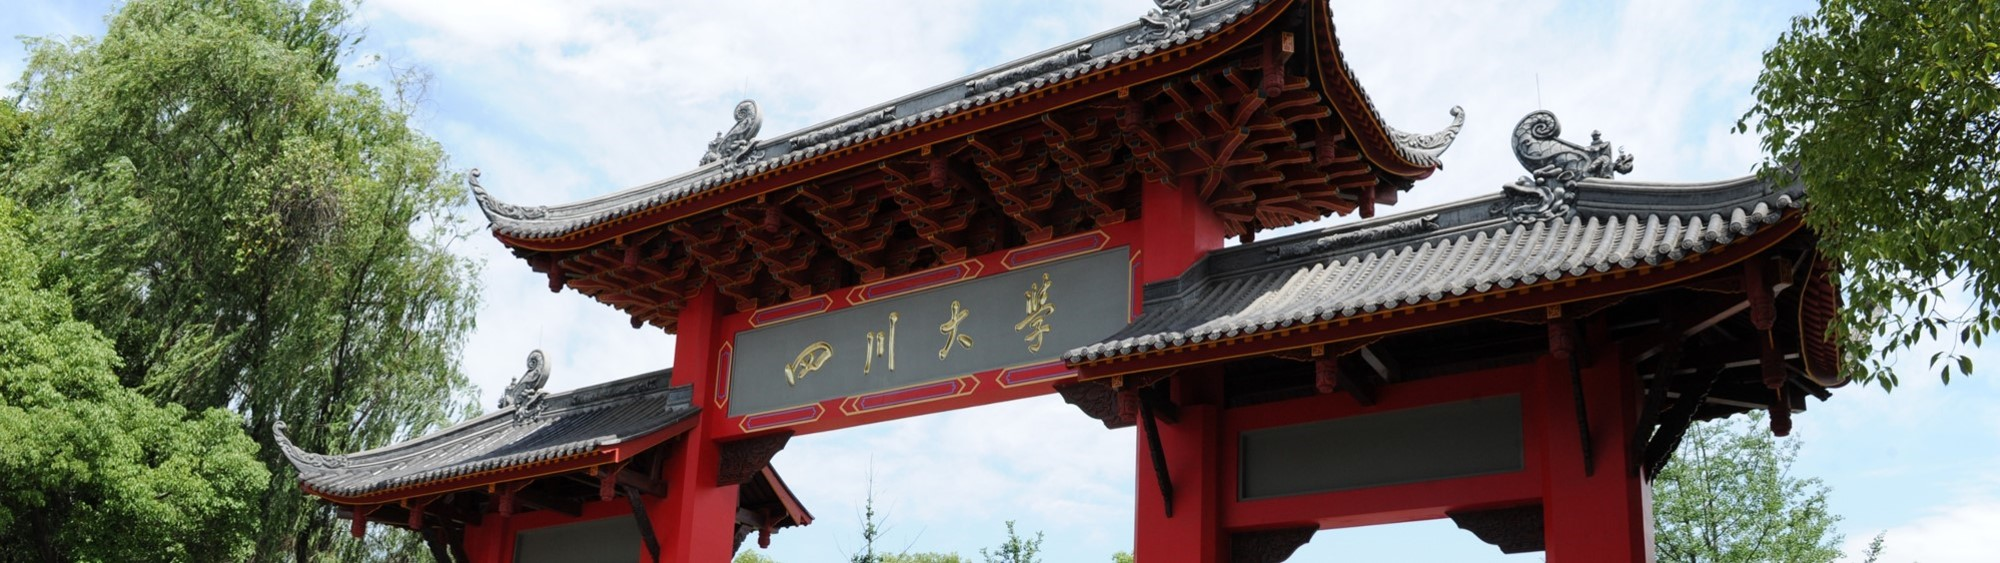
\includegraphics[width=\paperwidth,height=0.5\paperheight]{end.jpg}};
    }
\begin{frame}
\vspace{2.5cm}
此模板获得了来自GPT4的帮助 

感谢Texlive社区

感谢AR PL KaitiM GB字体的开发人员

感谢吴玉章学院宽松的环境让我有时间去探索自己未知的领域

\end{frame}}
\end{document}